%!TEX root = SysSpec_ClockPendulumAnalyzer.tex
\subsection{Umsetzung des Counters} %TODO Counter Realisierung beschreiben
Der Tick-Counter zwischen den Pendeldurchgängen basiert auf einem freilaufendem Zähler, welcher auf dem TinyK20 Mikrocontrollerboard läuft, getrieben von dem vorhandenen, termperaturkorrigierenden 8MHz Quarz.
Um die Schwankungen des Zählers auszugleichen wird der Sekundenpuls des GPS-Moduls über zwei unabhängige IO-Pins genutzt. Eine Leitung, für den Fall, dass keine GPS-Verbindung besteht, am FIX-Pin des GPS-Moduls angeschlossen und eine zweite Leitung, falls GPS-Verbindung besteht, am PPS-Pin des GPS-Moduls.\\
Beide Leitungen funktionieren über einen Interrupt der höchsten Priorität. Falls am PPS-Pin Interrupts eingehen, wird der FIX-Pin ignoriert. Beim Umschalten zwischen GPS-Empfang und keinem GPS-Empfang kann daher ein Fehler entstehen, weshalb, dann die nächsten Messwerte mit 0 belegt nach aussen gesendet werden, um diese Messung zu verwerfen.
Im Normalbetrieb werden die Interrupts an den IO-Pins, eingehend vom GPS-Modul, dazu genutzt die Differenz zwischen dem letzten Zählerwert und dem aktuellen Zählerwert zu bilden und so die effektive Frequenz zu ermitteln.\\ 
Die Pendeldurchgänge werden über einen weiteren IO-Pin über einen Interrupt der höchsten Priorität ermittelt. Dabei wird jede zweite Messung verworfen, um das Pendel immer von der gleichen Seite zu messen. Der ermittelte Zählerwert wird gemeinsam mit der ermittelten Frequenz gespeichert und bei Anfrage über die \iic\ Schnittstelle gesendet.\\
\\
GPS-Modul und TinyK20 sind auf einem Board gemeinsam angebracht, ebenfalls auf diesem Board befindet sich die RTC und er Anschluss für den Sensor für die Pendel-Registrierung (Abbildung \ref{fig:hardware_board}).
	\begin{figure}[H]
		\centering
		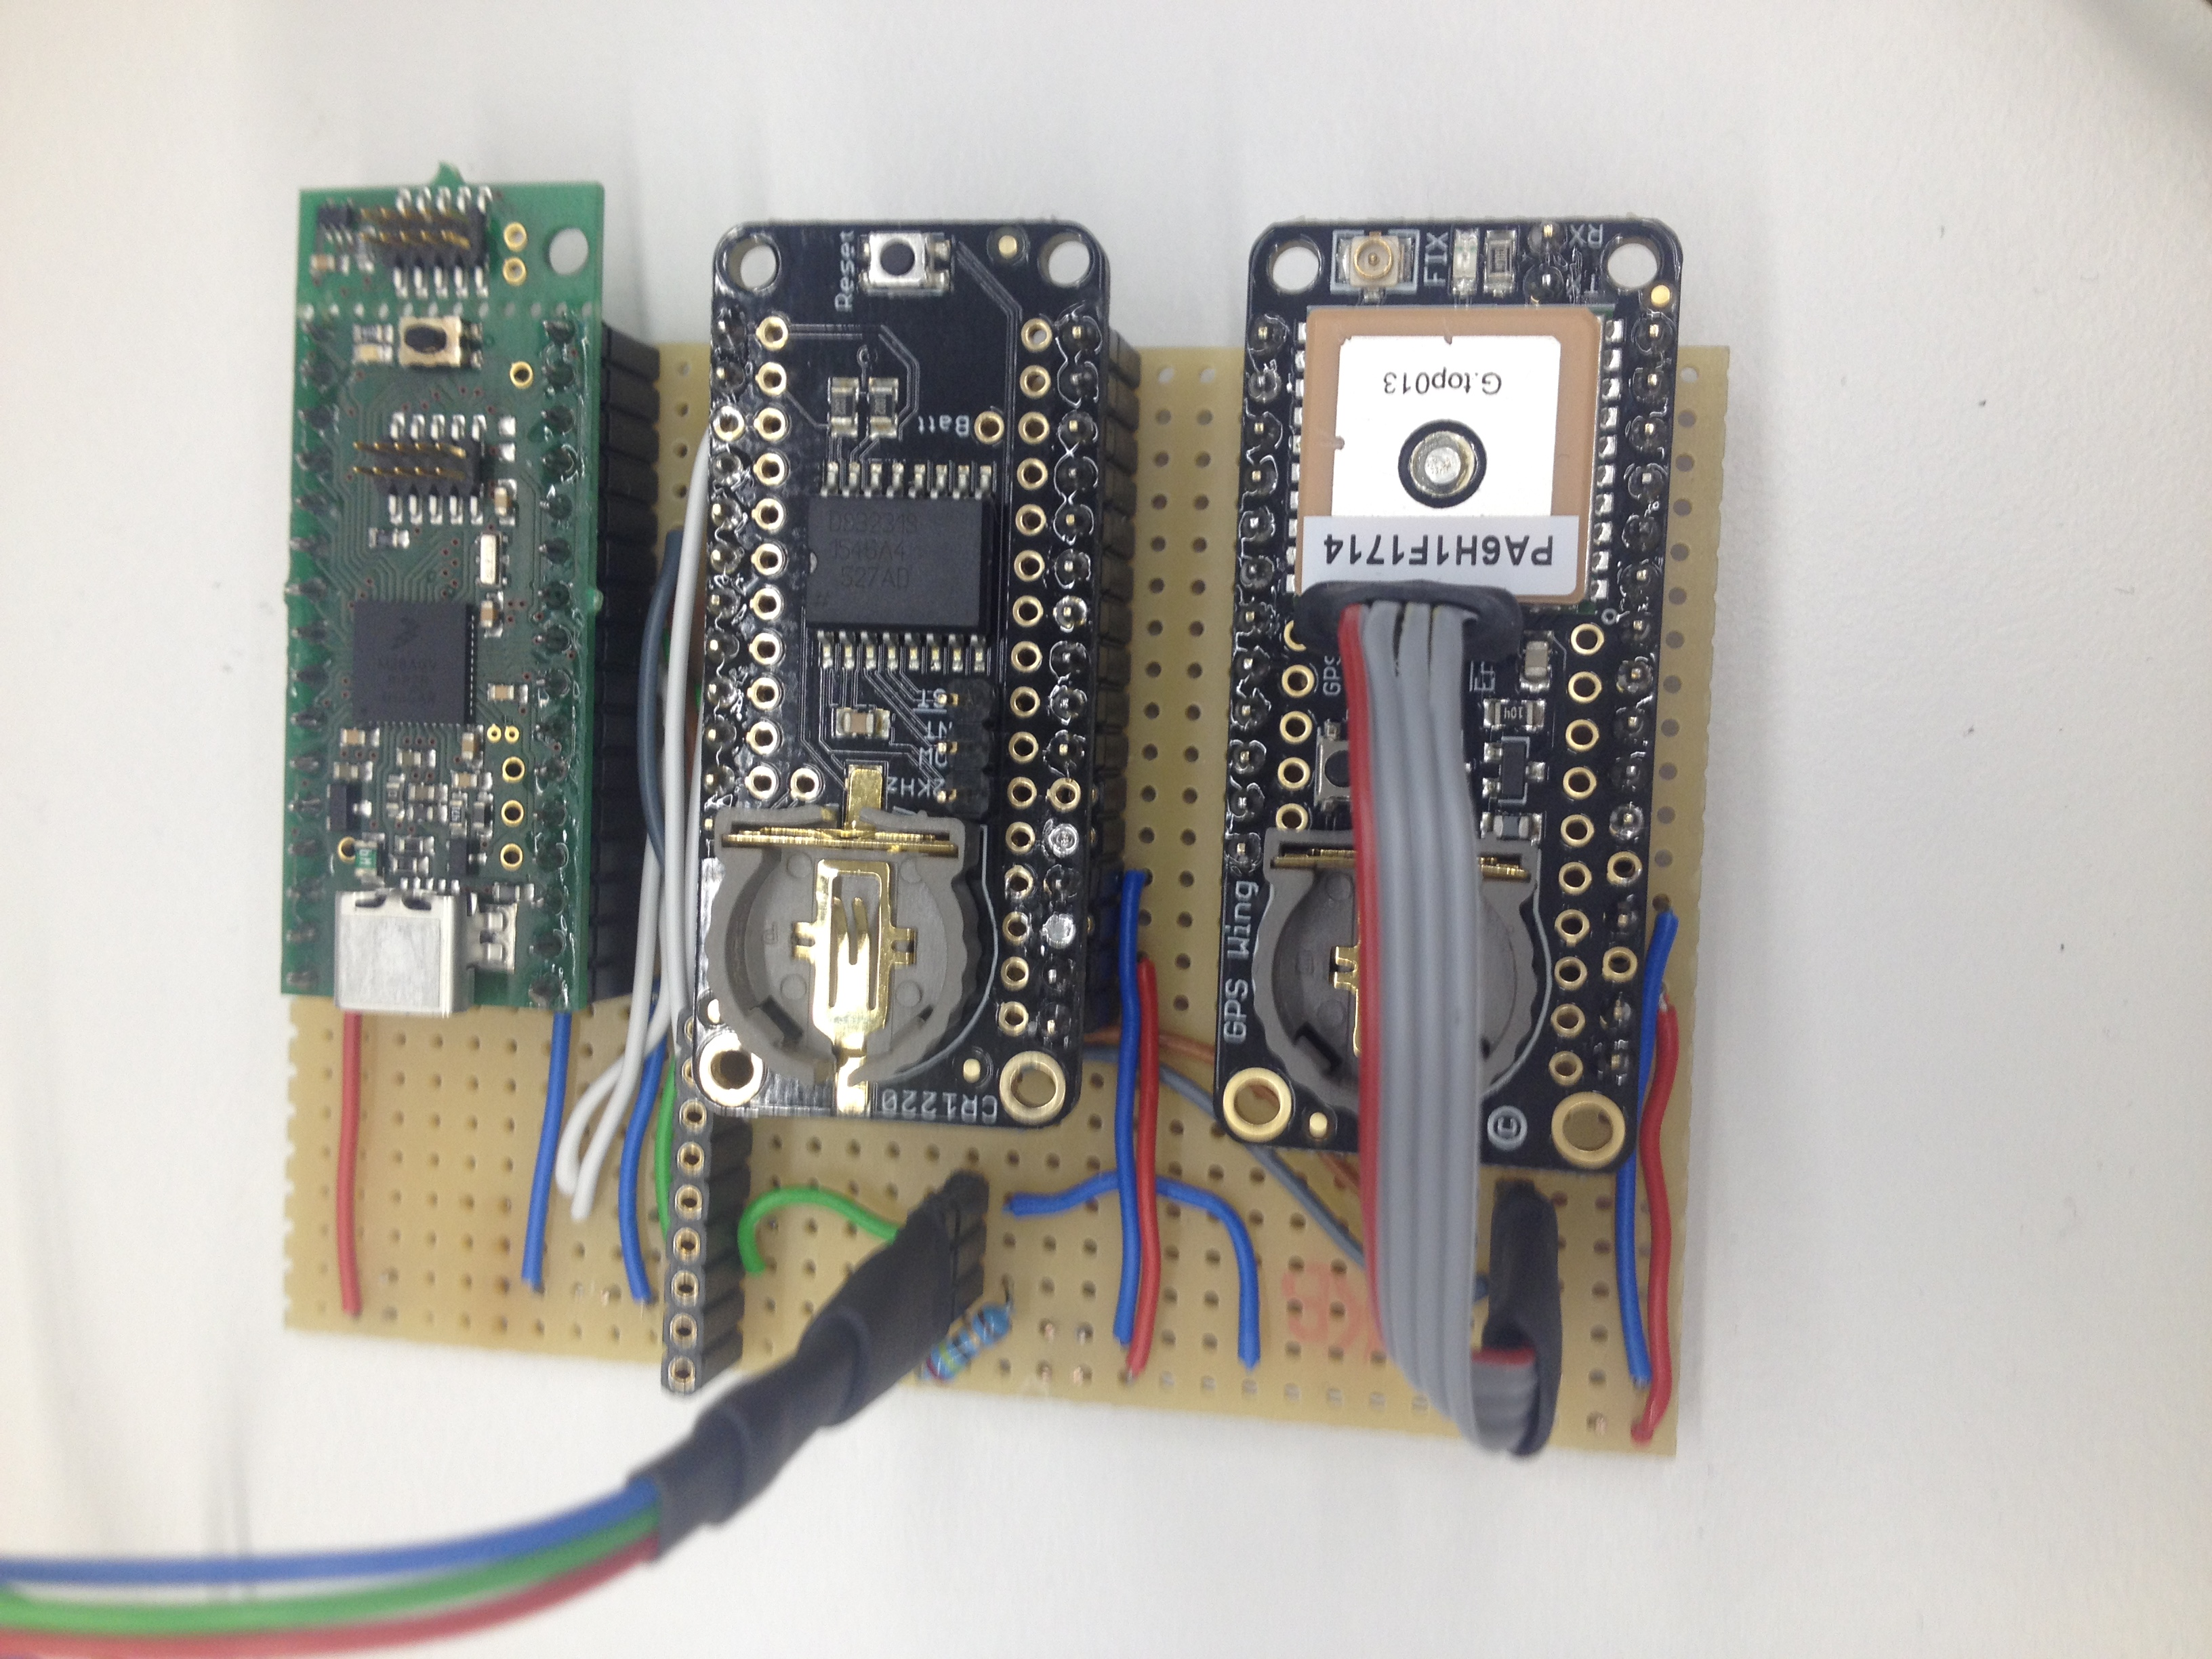
\includegraphics[width=.7\textwidth]{HW_Board_Complete}
		\caption{Gesamtanordnug der Hardware-Komponenten}
		\label{fig:hardware_board}
	\end{figure}